\section{Electro-pneumatic Implementation\label{sec:electropneumatic_implementation}}

Several steps were taken in the implementation phase with the pneumatic system to facilitate further understanding of the subsystems' dynamics, and to provide data and models that could be used in the implementation of controller software. A Simulink model was developed of the electro-pneumatic actuation system in order to verify that fundamental design would work and to gain further insight into the operation of the pneumatic system. A simple PID controller block was used to show that the closed-loop system was inherently stable.

\subsection{Simulation}

The top level of the Simulink model is shown in \ref{fig:pneumatics_top_level}: A PID controller block is used in a closed-loop configuration, and the response to a fixed step input is displayed on the scope block.

In modelling the electropneumatic system, 3 subsystems were identified and modelled independently:

\begin{enumerate}
  \item the PWM generator;
  \item the solenoid valves;
  \item and the pneumatic actuator (single-acting spring-return cylinder).
\end{enumerate}

\begin{figure}[h]
\centering
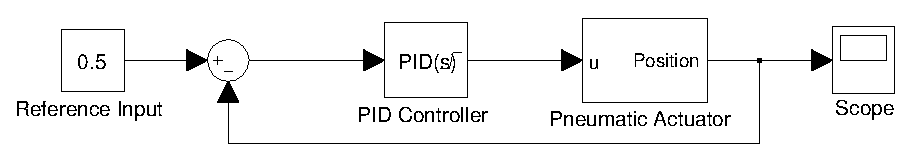
\includegraphics[scale=1]{implementation/figures/pneumatic_modelling1.eps}
\caption{Top-level electropneumatic model for simulation in Simulink.}
\label{fig:pneumatics_top_level}
\end{figure}

\paragraph{PWM Generator}

The PWM generator in Simulink was built using the instantaneous model presented by \citet{valve_models} which compares a generated saw-tooth signal, $V_{saw}$ with a period $T_{saw}$, with the input signal $V_{in}$ to obtain the pulse-width-modulated signal $U$:

\begin{equation}
\label{eq:pwm_generation}
U\left(t\right) = 
\begin{cases}
1 & V_{in}\left(t\right) \geq V_{saw}\left(t\right) \\
0 & V_{in}\left(t\right) < \left(t\right)
\end{cases}
\end{equation}

The Simulink model which implements Eq.\ \ref{eq:pwm_generation} can be seen in Fig.\ \ref{fig:pneumatics_pwm}. The input to the subsystem, shown as \emph{In1}, is $V_{in}$, and the output, shown as \emph{Out1} is the pulse width modulated signal $U$. A Saturation and block was added to limit the input signal $V_{in}$ to the range [0..1]. A dead zone block was added to simulate the effect of dead zone in the response of the solenoid valves to a PWM signal: if the pulse width is too short, the current through the solenoid cannot generate enough force to open the poppet, so the valve stays shut. This is a parameter of the solenoid valve, and was quantified experimentally by \cite{valve_models} as the minimum input signal $V_{in}$ required to open the valve at all. \Citet{accurate_position} also account for a minimum possible duty cycle in the solenoid valve input signal as

\begin{equation}
  \label{eq:pwm_duty_min}
  d_{min}=\left(T_{vr}/T_{PWM}\right)\cdot100\%
\end{equation}

where $T_{vr}$ is the valve response time, and $T_{PWM}$ the PWM period.


\begin{figure}[h]
\centering
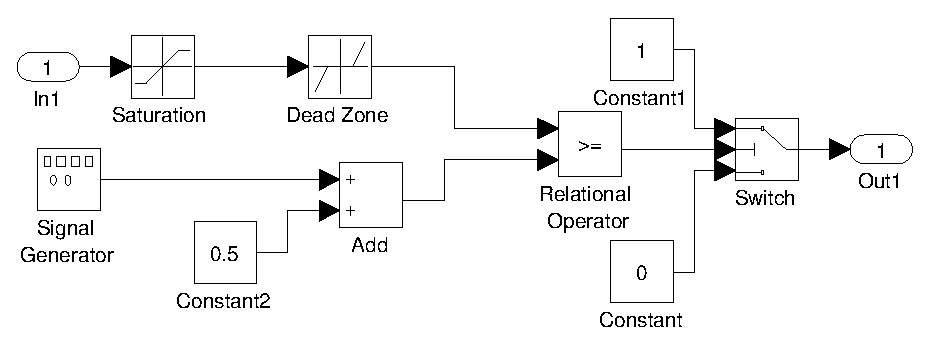
\includegraphics[scale=0.65]{implementation/figures/pneumatic_modelling2.eps}
\caption{Simulink PWM Generator model.}
\label{fig:pneumatics_pwm}
\end{figure}

The signal generator block in Fig.\ \ref{fig:pneumatics_pwm} outputs a triangle wave with peak-to-peak amplitude 1, which is then offset by 0.5. The relational operator block then compares this with the input signal, and outputs either a 1 or a 0.

\paragraph{Solenoid Valves}



\paragraph{Pneumatic Actuator}

The Simulink pneumatic actuator subsystem can be seen in Fig.\ \ref{fig:pneumatics_actuator}. In order to save time, pre-built Simulink blocks from the Simscape package were used to model the dynamics of the actuator. Physical port 1 (denoted by the octagonal port symbol) in \ref{fig:pneumatics_actuator} is the air inlet. Physical ports 2 and 3 are the displacement ports of the cylinder, and regular port 1 is used to display the displacement on a scope.

\begin{figure}[H]
\centering
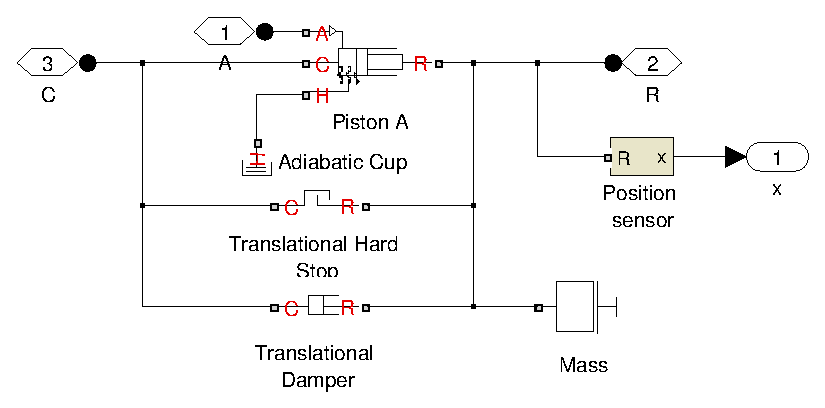
\includegraphics[scale=0.65]{implementation/figures/pneumatic_modelling3}
\caption{Simulink actuator model.}
\label{fig:pneumatics_actuator}
\end{figure}

\paragraph{Overall Electropneumatic Simulink Model}

The complete open-loop actuator model can be seen in Fig.\ \ref{fig:pneumatics_model_full}. The absolute value of the real-valued input $u$ is first fed to the PWM block. This signal is then converted into seperate signals for each of the two solenoid valves in a way similar to the first PWM pulsing scheme presented by \citet{accurate_position}. The input to the subsystem $u$ is expected to range from -1 to 1. When $u\geq0$, the input to valve A is  the pulse width modulated signal $U$, and the input to valve B is 0. When $u<0$, the opposite occurs.

\begin{figure}[H]
\centering
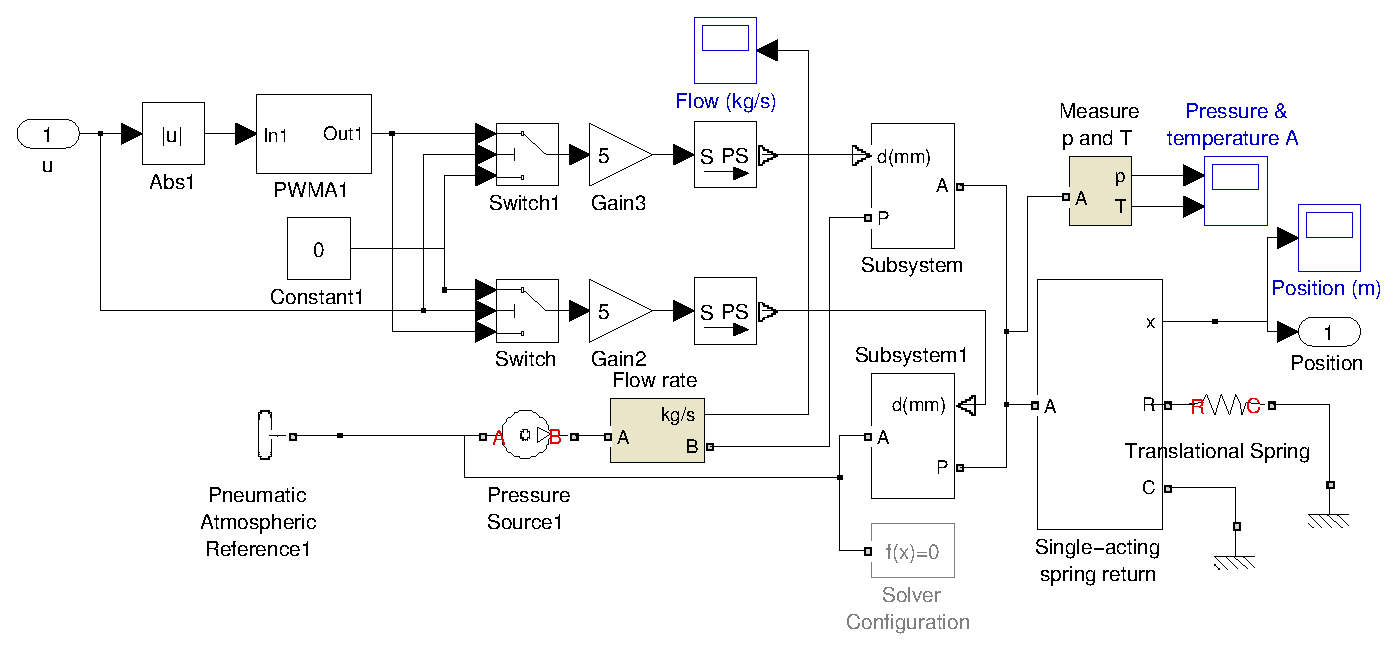
\includegraphics[scale=0.65]{implementation/figures/pneumatic_modelling4}
\caption{Overall electropneumatic model.}
\label{fig:pneumatics_model_full}
\end{figure}

\subsection{Solenoid Valves}

Solenoid valves and cylinders from SMC corp were chosen for a physical implementation of the design. The solenoid valve specified for a sample implementation is a \emph{VQZ115}-series, as shown in Fig.\ \ref{fig:smc_solenoid_valve}. Table \ref{tab:solenoid_specs} shows the specifications for this solenoid valve. Particularly of interest was a valve with a high flow coefficient, or $C_v$, which is an industry standard measure of the fluid flow efficiency of the valve.

\begin{table}[H]
  \caption{Solenoid valve specifications.\label{tab:solenoid_specs}}
  \centering

  \begin{tabular}{|l|l|}
  \hline
  Part & VQZ115-6L1-N1-PR \tabularnewline
  \hline
  Coil Voltage & \unit{12}{\volt} \tabularnewline
  \hline
  Configuration & 3-port normally closed \tabularnewline
  \hline
  Flow coefficient & $C_v=\unit{0.23}{}$ \tabularnewline
  \hline
  Max. Operating Frequency & \unit{20}{\hertz} \tabularnewline
  \hline
  Max. Pressure & \unit{0.7}{\mega\pascal} \tabularnewline
  \hline
  \end{tabular}
\end{table}

\begin{figure}[H]
\centering

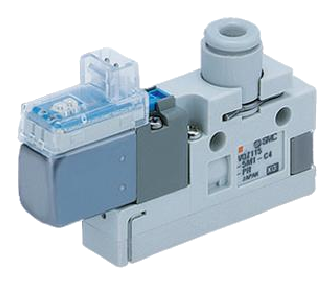
\includegraphics[scale=0.5]{implementation/figures/solenoid_valve.eps}
\caption{SMC solenoid valve.}
\label{fig:smc_solenoid_valve}
\end{figure}



\subsection{Pneumatic Actuators}


\subsection{Positional Feedback Sensors}


\subsection{Mechanical Linkage}
